\chapter{Einleitung}

Im Jahr 2022 veränderte OpenAI mit ihrem browser basierten ChatGPT (Generative Pre-trained Transformer) die welt komplett. In nur fünf Tagen erreichte ChatGPT die eine Millionen Nutzer und ist im Leben vieler Menschen Alltag und in manchen garnicht mehr weg zu denken.
Die GPT KI (Künstliche Intelligenz) von OpenAI gehört zu der Familie der LLMs (Large Language Models) oder auch MLLMs (Multimodal Large Language Models), wenn diese weitere Datenmodalitäten verarbeiten können wie zum Beispiel Bilder, Audi und Video.
Inzwischen haben LLMs von anderen Anbietern mit der Qualität und den Fähigkeiten von OpenAIs GPT gleichgezogen. Inzwischen gibt es viele Arten LLMs zu Bewerten und ein reger Wettbewerb ist um die vielen Bewertungen entstanden.
%https://doit.software/de/blog/chatgpt-statistiken#screen5

Die GPT Modelle von OpenAi und anderen Anbietern wie Google\'s Gemini sind nur über eine API (Programmierschnittstellen) meistens gegen Entgeltung verfügbar.
Open-Source Modelle wie Liang Wenfengs DeepSeek oder Metas LLAMA erfreuen sich immer größere beliebtheit da sie gratis auf der eigene Hardware ausgeführt werden können.

Im Oktober 2023 kam ich das erste mal mit RAGs (Retrieval-Augmented Generation) in Kontakt, damals war die Idee über mehrer Firmeninterne Informationsquellen mithilfe eines LLMs Fragen zu beantworten.
Bei einem Hackathon gelang es uns einen Prototypen zu entwickeln der mit einem gewissen Erfolg Fragen zu Firmeninternen Themen beantworten konnte.

Einer der Schritte während der Entwicklung war das ständige Testen der neusten Änderungen um zu gucken, ob das System noch funktioniert und oder wie es sich verschlechtert hat.
Das war schon damala immer relativ Mühselig und raubte uns wertvolle Zeit diese Bewertungen vor zu nehmen.
Gerne hätten wir unterscheidliche Promts inerhalb unseres Systems getestet oder automatisch eine überprüfung unseren neusten Änderungen gehabt.

RAGAs wurde entwickelt um diese Probleme zu lösen, es hat zudem das Alleinstellungsmerkmal, dass man weder eigen Fragen noch die genereierten Fragen selber beantworten muss.
Sowohl die generierung eines Fragenkataloges (Testsets) als auch die Beantwortung der Fragen um eine Musterlösung zu haben nimmt RAGAS mit hilfe von LLMs vor.
Mithilfe dieses Testsets und von RAGAS eigens Entwickelten Metriken welche die wichtigsten Funktionen eines RAGs abdecken kann dann eine Bewertung des Systems vorgenommen werden.

Damit benutzt RAGAS die neue LLM Technologie um das durch LLMs entstandene System sleber zu testet. Dies spart viele Menschliche Resourcen welche Zeit und Kostenintensiv sind.

\section{Wie funktioniert ein RAG}

\begin{quote}
    Bei Retrieval Augmented Generation (RAG) erweitert man den Prompt für das LLM um Suchergebnisse aus einer Dokumentensammlung, einer Datenbank, einem Wissensgraf (Knowledge Graph) oder einer anderen Suche (z.B. Internetsuche). Das Wissen für die Antwort kommt also aus angebundenen Quellen und nicht aus dem LLM.
\end{quote}
\cite{honroth2024retrieval}\\ \\

\begin{figure}[h!]
    \centering
    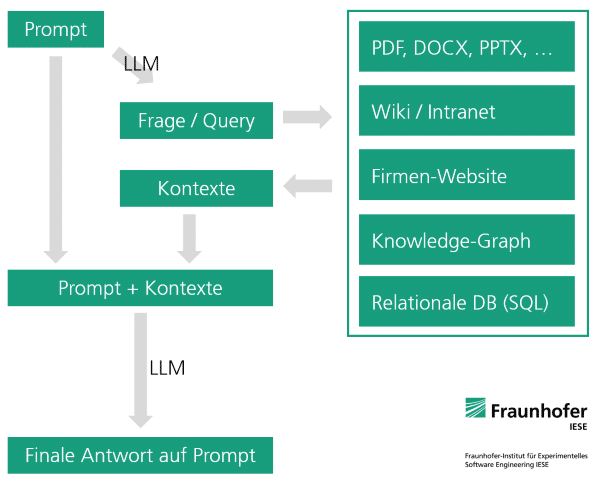
\includegraphics[width=0.5\textwidth]{retrieval_augmented_generation_RAG_600px.png}
    \caption{Struktur eines RAGs, Quelle: \cite{honroth2024retrieval}}
    \label{fig:Rag Structure}
\end{figure}


\subsection{Vorteile von RAGs}
Bei der Wissenabfrage durch LLMs zeigen sich unter anderem folgende Schwachstellen:
\begin{enumerate}
    \item Im Trainingsset für die LLMs selten vorkommendes Wissen können selbst LLMs schlecht lernen. \cite{gao2023rtre} \cite{press2022measuring}  
    \item LLMs haben einen gewissen Wissensstand und müssen weiter trainiert werden, um die neuesten Informationen zu kennen.
    \item Firmen interne Dokumente sind nicht im Trainingsset und daher können LLMs keine Fragen zu Firmen Internen Daten beantworten.
\end{enumerate}

Die Nutzung eines RAGs ist eine der drei Möglichkeiten, um ein LLM zu verbessern.
RAGs haben neben dem Fine-Tuning und dem nutzen eines LLMs mit großem Sichtfenster entscheidende Vorteile.

Es gibt einige Faktoren, welche die Entscheidung beeinflussen können, ob ein RAG besser für den betrieblichen Ablauf geeignet ist.
Die Kompetentz der Betreiber des RAGs, die Art der Daten und die Fianziellen Möglichkeiten des Unternehmens


\subsection{Kompetenz des Betreibers}
Für das Finetuning von LLMs ist ein gewisses technisches Wissen notwendig, um die Themen Natural Language Processing (NLP), Deep Learning, Modellkonfiguration, Datenaufbereitung und Evaluierung anzuwenden.
Der gesamte Prozess des Finetunings ist technisch Anspruchsvoll, erfordert das Sichten der neuen Trainingsdaten und ist zudem durch die benötigte Hardware teuer.

Das benutzten eines LLMs benötigt die geringste Kompetenz des Betreibers da hier das LLM unverändert bleibt. Hier werden einfach die Daten inklusive der Frage an das LLM gesendet.

Während das LLM in einem RAG auch unverändert bleibt wird es in ein System mit mehreren Komponenten eingebunden.
Hier ist ein allgemeines Verständniss von LLMs und effektiven Methoden für den suchenden (Retrival) Teil des RAGS notwendig.
Zudem müssen hier manuell für jeden Datentypen (Email, PDF etc.) angebunden werden. Sollte ein seltender Datentyp verwendet werden muss hier eventuell eigens eine Anbindung entwickelt werden. 
\subsection{Datenbasis}
Sollten die Daten dynamisch sein, ist das RAG die vorzuziehende Lösung. Durch die Eigenschaften der schnellen und kontinuierlich aktualisierung der Daten.
Wie vorhin erläuter kann es jedoch sein, dass es schlechte oder keine Unterstützung von selten verwendeten Dateiformaten gibt.

Der Prozess des Finetunings erstellt hingegen eine Momentaufnahme, die ein erneutes Training erfordert.
Beim Finetuning ist es möglich, dass das Modell Muster erkennt und firmeneigene Begriffe verstehen kann, dies ist ein deutlicher Vorteil gegenüber den anderen Methoden.


\subsection{Budget}
Das Finetuning erfordert für lange Zeit teure Rechenzeit auf Hochleistung-GPUs, was das Training eines Modells kostenintensiv macht.

Das RAG verursacht dagegen zusätzliche Kosten durch das Speichern der Daten in einer Vektordatenbank.

Die wohl kostenintensivste Methode ist das nutzen eines LLMs mit einer großen Context Window.


\section{Objektive Beurteilung von RAGs}
Je mehr Daten einem RAG zur Verfügung stehen, desto aufwendiger ist es, die Qualität des RAGs zu beurteilen.
Eine Beurteilung durch Menschen müsste bei Anpassungen am RAG oder Änderungen an den Daten neu durchgeführt werden.

Tools wie RAGAS, die bereits eine automatisierte Bewertung versuchen, diesen Prozess unter anderem mithilfe von LLMs zu automatisieren.
Diese Tools generieren aus den ihnen gegebenen Daten Fragebögen, die auf eine Frage eine beispielhafte Antwort und die genutzten Stellen aus den vorher gegebenen Dokumenten beinhalten.
Sollten nach diesem automatisierten Test die gewünschten Ergebnisse nicht erreicht werden, kann zum Beispiel die Veröffentlichung blockiert werden.

Sowohl menschliche Bewertungen als auch die reine subjektive Bewertung durch LLMs sind jedoch nicht objektiv.
Anhand mehreren Techniken kann versucht werden, die Bewertung mithilfe von LLMs zu objektivieren.

\section{Darstellung des Themas und der Forschungsfragen}
In dieser Bachelorarbeit wird untersucht, wie gut diese Tools sowohl subjektive als auch objektive Bewertungen durchführen können.
Im Mittelpunkt werden die beiden Tools RAGAS und Giskard stehen, welche die Bewertung durchführen.


\section{Praxistauglichkeit und Herausforderungen}
Es stellen sich mehrere Herausforderungen für die Bewertung von RAGs durch diese Tools.
\begin{itemize}
    \item Die Kosten, die bei der Bewertung entstehen.
    \item Die Zeit, welche es dauert, die Bewertung durchzuführen, die Bewertung kann schneller durchgeführt werden kann, wenn mehr Ressourcen zur Verfügung stehen.
    \item \item Das aufsetzten des zu testenden Systems. Dies beinhaltet eine eventuelle doppelte Speicherung der Daten und die für das Testen benötigten Aufrufe des LLMs.
    \item Das System muss auch auf dem neuesten Stand gehalten werden, da sich dieses noch relativ junge Thema schnell entwickelt.
\end{itemize}

\section{Softwaretechnische Fragestellungen}

In dem Artikel \textit{RAG in der Praxis – Generierung synthetischer Testdatensätze} untersucht Luka Panic~\cite{pixion2024rag} die Testset generierung mithilfe von RAGAS. Es treten bei 17 \% der generierten Fragen Fehler beim Generieren der Testfragen auf.
Dies hat vielfältige Gründe, die von nicht verwertbaren Antworten des LLMs bis zu Verbindungsproblemen oder dem Erreichen des Limits der maximalen Anfragen an APIs reichen.

Auch bei der Bewertung von Antworten können sich ungewollte und bisher noch ungeahnte Biases einschleichen. In diesem Paper \cite{yang2023llmfairness} wird gezeigt, dass, wenn ein LLM eine von zwei gegebenen Antworten aussuchen müsste, die erste bevorzugt wurde, selbst wenn die gleiche Frage mit anderer Reihenfolge gestellt wurde.
RAGs vergleicht keine Antworten miteinander und daher ist dieser Bias kein direktes Problem für uns. Was jedoch einen Einfluss auf die Bewertung von Antworten haben kann, ist der Bias zu gewissen Nummern.
Wie in \cite{shaikh2024cbeval} beschrieben, bevorzugen LLMs bei der Bewertung lieber Zahlen, welche Mehrfache von 5 und 10 sind.

Auch die allgemeine stochastische Natur von LLMs spielt eine Rolle, da bei der gleichen Anfrage unterschiedliche Antworten und dadurch auch Bewertungen zurückgegeben werden. Wie groß diese Abweichungen sind, wird in dieser Arbeit kurz untersucht.

Wie in diesem Paper \cite{gemini2024v15} beschrieben, stellt Gemini 1.5 einen bedeutenden Fortschritt in der multimodalen Verarbeitung großer Kontextfenster dar. Das wirft auch die Frage auf, ob RAGs nicht irrelevant sind und durch LLMs mit großen Kontextfenstern abgelöst werden.
Es gibt einige Gründe, die dagegen sprechen: LLMs mit größeren Kontextfenstern werden immer langsamer und teurer, die genauen Kosten sind abzuwarten. Jedes Mal alle Daten in den Kontext zu laden, besonders wenn dies über das Internet geschieht, ist eine weitere Hürde. LLMs fällt es auch schwer, bei zu vielen Informationen noch die relevanten zu finden, was zu schlechteren Antworten führen kann.
Diese Faktoren lassen darauf schließen, dass RAGs, die nicht nur eine einfache Suche nutzen, noch länger relevant bleiben.

% Kann ich hier wirklich Diskussionen von Twitter linken oder mache ich mich dann lächerlich?
% https://x.com/agishaun/status/1758561862764122191
% https://x.com/ptsi/status/1758511315646320920

https://huggingface.co/PleIAs/Pleias-RAG-1B


Pitfalls in LLM Assisted Evaluation https://medium.aiplanet.com/evaluate-rag-pipeline-using-ragas-fbdd8dd466c1

\section{Rechtliche Fragestellungen}

Am 01.08.2024 trat die Verordnung über Künstliche Intelligenz der Europäischen Union (KI-VO) in Kraft. Die Verordnung setzt Regelungen und Maßstäbe für die Verwendung von KI.
RAGs sind gemäß Artikel 3 Nr.1 KI-VO KI-Systeme und fallen damit in den Anwendungsbereich der KI-VO.
Bei der Nutzung oder Bereitstellung von LLMs muss sich an die KI-VO gehalten werden. Die Nutzer*innen der RAGs müssen sich den aus der KI-VO ergebenden Pflichen bewusst sein, wie bei der Verwendungun von vertraulichen Daten.


% Einer der wichtigen Faktoren bei der Nutzung von LLMs ist zudem die rechtliche Lage, dafür hat die EU die KI-Verordnung erlassen. Diese regelt wichtige Fragen und sorgt für eine notwendige Dokumentation bei gewissen Modellen.

% Dabei sind für RAGs folgende EU-KI-Verordnungsunterscheidungen interessant: Bereitstellungsform und der Sektor.

% Bei der Bereitstellungsform gibt es drei Stufen, kommerziell, Open-Source, intern.\\
% Bei kommerziellen LLMs wie GPT-4 wird in § 53 geklärt, welche Dokumentation die Anbieter bereitstellen müssen, dies ist besonders bei B2B Geschäften wichtig.
% Sollte also das Unternehmen das RAG nach außen hin für z. B. Kunden zugänglich machen, ist dies eine rechtliche Absicherung.\\
% Open-Source-Modelle werden von diesen Regularien in § 53 (2) befreit, unter der Annahme, dass sie nicht als systemisches Risiko eingestuft werden.
% Modelle werden dann als systemisches Risiko eingestuft, wenn Sie eine gewisse „Größe/Qualität" erreichen. \\
% Die allermeisten aktuell zur Verfügung stehenden Modelle fallen nicht in diese Ausnahme und 

% Bei einer rein internen Nutzung des LLMs kann auch gut ein Open-Source LLM verwendet werden, welches eine komplett interne Speicherung von Daten ermöglicht.

% Auch zu beachten ist der Sektor, sollte dieser ein Hochrisiko-Bereich sein, wie in der Justiz oder den Finanzen, wo das RAG und damit das LLM Vorschläge macht, dann muss dies gewisse Auflagen erfüllen.
% Da hier aber nicht nur das LLM, sondern auch der Rest des Systems wie die Vektor-Datenbank allgemein strengen Auflagen unterliegt, ist dies dann nur ein weiter Tropfen auf den heißen Stein?


%\textbf{Open-Source-Modelle} (z.B. Llama 2, Mistral 7B, Deepseek R1) bieten eine Vielzahl von Vorteilen, wie die Möglichkeit, sie zu modifizieren und mehr Kontrolle über die Daten zu haben, was rechtliche Vorteile bietet, aber auch Nachteile. Entscheident ist zudem wieder die Technische Kompeten welche benötigt wurd um diese Modelle selber zu Hosten.\\
%\textbf{Mittelklasse-API-Modelle} (z.B. Claude Haiku, GPT-3.5 Turbo) sind günstiger als die Hochleistungsmodelle und bieten dennoch eine gute Leistung. Da sie nicht Open Source sind, bieten sie weniger Kontrolle über die Daten und das Modell selbst. Manchmal muss man mehr für private Instanzen zahlen.\\
%\textbf{Hochleistungsmodelle} (z.B. GPT-4, Claude 3 Opus) sind die teuerste Option, bieten aber auch die beste Leistung, sowohl in Bezug auf Geschwindigkeit als auch auf die Qualität der generierten Antworten. Sie haben ähnliche Vor- und Nachteile wie die Mittelklasse-API-Modelle.\\

